% Drawing 57/08-6 -- folder 57, batch 08, archive page 154 (PDF page 155).
% Transcription: plusieurs configurations de composantes concourantes ; une boucle à point double ; un arc portant un point épaissi
% Kind: page of sketches of curves. Method 2 (schematic redraw from the facsimile). Status: partial.
% Notes: Lower half of the page: about eight configurations of concurrent or crossing lines (some with a heavy point at the meeting), one inside a bracket-like arc; a loop with a double point beside nu_s >= 3; a thick arc carrying a thickened point. The configurations are schematic: the number and direction of strokes in the denser ones are approximate. The formula in the upper right (2(c_0 + rho) - ...) is text and is left out.
% Coordinates: 1 unit = 1 mm = 1/100 of the crop width (bbox in page fractions: [0.1, 0.53, 0.95, 0.87]).
% Redrawn by Claude (claude-opus-5-5), issue #73, 2026-11-07; not checked by a human; not compiled (no TeX in the session).
% Rights: reproduces part of the work -- behind RENDER_TRANSCRIPTS, never published by itself.
\documentclass[tikz,border=3pt]{standalone}
\usepackage{amsmath,amssymb}
\usetikzlibrary{patterns,arrows.meta}
\tikzset{pencil/.style={black!45}, struck/.style={black!35}, mark/.style={circle,draw,inner sep=1.3pt}, pt/.style={circle,fill,inner sep=0.9pt}, opt/.style={circle,draw,fill=white,inner sep=1.1pt}}
\begin{document}
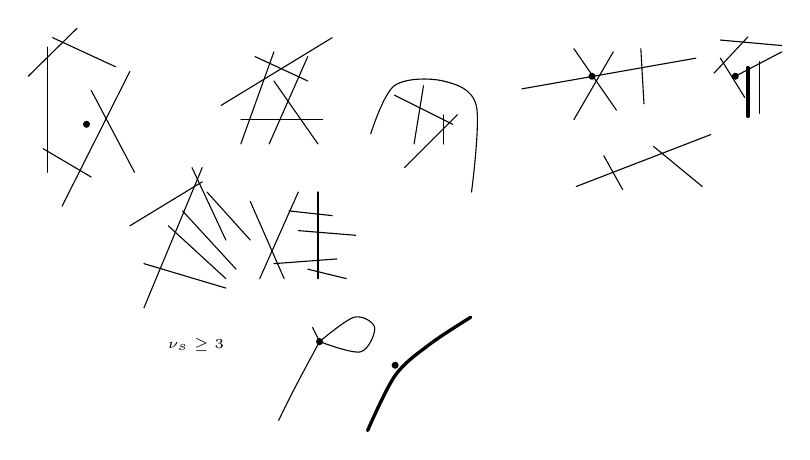
\begin{tikzpicture}[x=1mm,y=1mm,line cap=round,line join=round,font=\scriptsize]
\draw (2.4,-9.8) -- (8.6,-3.7);
\draw (5.5,-4.9) -- (13.5,-8.6);
\draw (4.9,-6.1) -- (4.9,-22);
\draw (10.4,-11.6) -- (15.9,-22);
\draw (15.3,-9.2) -- (6.7,-26.3);
\draw (4.3,-19) -- (10.4,-22.6);
\node[pt] at (9.8,-15.9) {};
\draw (26.9,-13.5) -- (41,-4.9);
\draw (31.2,-7.3) -- (37.9,-10.4);
\draw (33.6,-6.7) -- (29.4,-18.4);
\draw (29.4,-15.3) -- (39.8,-15.3);
\draw (33.6,-10.4) -- (39.2,-18.4);
\draw (33,-18.4) -- (37.9,-7.3);
\draw plot[smooth, tension=0.55] coordinates {(45.9,-17.1) (48.9,-11) (55.1,-10.4) (59.3,-13.5) (58.7,-24.5)};
\draw (48.9,-12.2) -- (56.3,-15.9);
\draw (52.6,-11) -- (51.4,-18.4);
\draw (50.2,-21.4) -- (56.9,-14.7);
\draw (55.1,-14.7) -- (55.1,-18.4);
\draw (15.3,-28.8) -- (24.5,-23.2);
\draw (23.2,-21.4) -- (27.5,-30.6);
\draw (17.1,-33.6) -- (27.5,-36.7);
\draw (20.2,-28.8) -- (27.5,-35.5);
\draw (22,-26.9) -- (28.8,-34.3);
\draw (25.1,-24.5) -- (30.6,-30.6);
\draw (24.5,-21.4) -- (17.1,-39.2);
\draw (30.6,-25.7) -- (34.9,-35.5);
\draw (36.7,-24.5) -- (31.8,-35.5);
\draw (35.5,-26.9) -- (41,-27.5);
\draw (39.2,-24.5) -- (39.2,-35.5);
\draw (33.6,-33.6) -- (41.6,-33);
\draw (36.7,-29.4) -- (44,-30);
\draw (37.9,-34.3) -- (42.8,-35.5);
\draw (65.1,-11.4) -- (87.2,-7.5);
\draw (71.7,-6.3) -- (77.1,-14.1);
\draw (76.7,-6.7) -- (71.7,-15.3);
\node[pt] at (74,-9.8) {};
\draw (80.2,-6.3) -- (80.6,-13.3);
\draw (90.3,-5.2) -- (98.1,-5.9);
\draw (89.5,-9.4) -- (93.8,-4.8);
\draw (90.3,-7.5) -- (93.4,-12.5);
\draw (92.2,-9.8) -- (98.1,-6.7);
\draw[very thick] (93.8,-8.7) -- (93.8,-14.9);
\draw (95.3,-7.9) -- (95.3,-14.5);
\node[pt] at (92.2,-9.8) {};
\draw (72,-23.8) -- (89.1,-17.2);
\draw (75.5,-19.9) -- (77.9,-24.2);
\draw (81.8,-18.7) -- (88,-23.8);
\draw plot[smooth, tension=0.55] coordinates {(34.2,-53.5) (36.4,-49.1) (39.4,-43.5)};
\draw plot[smooth, tension=0.55] coordinates {(39.4,-43.5) (43.8,-40.4) (46.4,-41.7) (44.6,-44.8) (39.4,-43.5)};
\draw (39.4,-43.5) -- (38.5,-41.7);
\node[pt] at (39.4,-43.5) {};
\node[inner sep=1pt] at (23.7,-43.9) {\tiny $\nu_s\geq 3$};
\draw[very thick] plot[smooth, tension=0.55] coordinates {(45.5,-54.8) (49,-47.8) (53.3,-43.9) (58.6,-40.4)};
\node[pt] at (49,-46.5) {};
\end{tikzpicture}
\end{document}
